\documentclass[american]{emisa}

\usepackage{todonotes}



\newcommand{\noteSM}[1]{\todo[color=red!40, author=\textbf{Salvador}, inline, caption={}]{#1}}
\newcommand{\noteJC}[1]{\todo[color=pink!40, author=\textbf{JC}, inline, caption={}]{#1}}
\newcommand{\noteSylvain}[1]{\todo[color=green!40, author=\textbf{Sylvain}, inline, caption={}]{#1}}
\newcommand{\noteAntoine}[1]{\todo[color=yellow!40, author=\textbf{Antoine}, inline, caption={}]{#1}}
\newcommand{\noteFabien}[1]{\todo[color=orange!40, author=\textbf{Fabien}, inline, caption={}]{#1}}
\newcommand{\noteJoel}[1]{\todo[color=blue!20, author=\textbf{Joel}, inline, caption={}]{#1}}

\newcommand{\mpc}{MULTI process challenge\xspace}

\usepackage{listings}
\usepackage{xcolor}
\usepackage{hyperref}
\usepackage{tikz-uml}

%\usepackage{amsmath,mathtools}%amssymb,
\usepackage{algorithmic,algorithm}

\definecolor{codegreen}{rgb}{0,0.6,0}
\definecolor{codegray}{rgb}{0.5,0.5,0.5}
\definecolor{codepurple}{rgb}{0.58,0,0.82}
\definecolor{backcolour}{rgb}{0.95,0.95,0.92}

\DeclareTextFontCommand{\mytexttt}{\ttfamily\hyphenchar\font=45\relax}

\lstdefinestyle{mystyle}{
    backgroundcolor=\color{backcolour},   
    commentstyle=\color{codegreen},
    keywordstyle=\color{magenta},
    numberstyle=\tiny\color{codegray},
    stringstyle=\color{codepurple},
    basicstyle=\ttfamily\footnotesize,
    breakatwhitespace=false,         
    breaklines=true,                 
    captionpos=b,                    
    keepspaces=true,                 
    %numbers=left,                    
    numbersep=5pt,                  
    showspaces=false,                
    showstringspaces=false,
    showtabs=false,                  
    tabsize=2
}

\lstset{style=mystyle}

\begin{document}
\begin{article}{
    % \title{\mpc: the FML solution}
    \title{Multi-level modelling with Openflexo/FML - A contribution to the \mpc}

    %% or include affiliations in footnotes:
    \author*{Sylvain Guérin}{firstname.lastname@ensta-bretagne.fr}
    \address{ENSTA Bretagne, Lab-STICC, UMR 6285, Brest, France}
    % \ead{firstname.lastname@ensta-bretagne.fr}

    \author{Joel Champeau}
    \address[a]{}

    \author{Jean-Christophe Bach}
    \address{IMT Atlantique, Lab-STICC, UMR 6285, 29238 Brest, France}
    % \ead{firstname.lastname@imt-atlantique.fr}

    \author{Salvador Mart\'inez}
    \address[b]{}

    \author{Antoine Beugnard}
    \address[b]{}

    \author{Fabien Dagnat}
    \address[b]{}

    \abstract{TODO, deadline = 31/05/2021

}
    \keywords{Multilevel Modeling Challenge, Federation Modeling Language, Openflexo}
    \bibliography{biblio.bib}
}

\section{Introduction}
\label{sec:introduction}
Model-driven engineering (MDE) has traditionally adopted a strict hierarchical two-level approach, where metamodels reside in a certain meta-level, and models are created one meta-level below by using types from the metamodel. Notable examples of this approach are the widespread Eclipse Modeling Framework (EMF)~\citep{emf} and the Object Management Group Meta-Object Facility(MOF)~\citep{omg2013mof}.

This strict approach shows its limitations when modeling complex domains requiring more than one level of specialization, e.g., to adapt the model to application sub domains. Indeed, the two-level approach fails to acknowledge and support: 1) the existence of different forms of classification and/or instantiation (e.g., ontological vs linguistic); and 2) the duality type-object for model elements. Therefore, while it may still be used for the aforementioned complex modeling tasks, the strict approach entails the introduction of accidental complexity in both the modeling process and the resulting modeling artefacts. 

In order to tackle this problem, the \emph{multi-level} modeling paradigm have been introduced. Contrary to the strict approach, multi-level modeling advocates the use of a flexible number of levels as well as a flexibilization of the relations between them. This paradigm is gaining traction lately within the modeling community as evidenced by the contribution of many new multi-level modeling approaches and tools such as Melanee~\citep{melanee}, MetaDepth~\citep{metadepth}, MultEcore~\citep{multecore2016}, DeepTelos\citep{deeptelos2016} or DMLA~\citep{dmla2017}. Taking advantage of this vibrant state of affairs, and in order to foster discussion and enable comparison between competing approaches, a multi-level modeling challenge has been created. This paper is a response to the latest multi-level modeling challenge
which consists in providing a solution to the problem of specifying and enacting processes. Solutions to the \emph{Multi-level Process Challenge} must fulfill a number of requirements for a process representation defined at an abstract process-definition level and at various more concrete domain-specific levels, resulting in a multi-level hierarchy of related models. We provide a solution based on model federation~\citep{Golra2016-federation}.

Model federation is a multi model management approach based on the use of virtual models and loosely coupled links. The models in a federation remain autonomous and represented in their original technological spaces whereas virtual models and links serve as control components used to present different views to the users and maintain synchronization. Our solution is based on this model federation infrastructure, namely, the use of virtual models and links. Concretely, we use OpenFlexo and its internal Flexo Modeling Language (FML), a language to create, link and manage virtual models, in order to achieve our goal. Our solution, which is fully implemented and executable, meets all the requirements.

%Links among models can be within a same level of abstraction or across levels of abstractions which gives, 

%as our answer to the challenge shows, a great flexibility.

The rest of the paper is organized as follows. Section~\ref{sec:technology} presents our approach and the technology it relies on. Section~\ref{sec:analysis} is the analysis of the problem. We detail our model in section~\ref{sec:model} and show it satisfies the challenge requirements in section~\ref{sec:requirements}. We assess the modeling solution in section~\ref{sec:discussion}. Section~\ref{sec:relatedwork} presents the related work before the conclusion.%~\ref{sec:conclusions}.


% \cite{multiProcessChallenge2019}

% \emph{Submissions responding to the challenge should describe
% a multi-level model conforming to the case description,
% including justifications for non-trivial design decisions. In
% order to foster comparability between solutions, respondents
% are asked to make sure that concepts of the case description
% are explicitly represented by one or more model elements.}\\

% \emph{criteria:
% \begin{enumerate}
%     \item Does the response address the established domain as described in the challenge description and demonstrate the use of modeling features?
%     \item Does it evaluate/discuss its proposed modeling solution against the criteria described in the challenge description?
%     \item Does it discuss the merits and limitations of the employed modeling technique?
%     Authors are invited to suggest further requirements to demonstrate particular benefits of the approaches they adopt.
% \end{enumerate}
% }

% structure : plus ou moins imposée par le challenge (structure actuelle = sections au moins attendues) 

%\noteSM{test}
%\noteJC{test}
%\noteSylvain{test}
%\noteAntoine{test}
%\noteFabien{test}
%\noteJoel{test}

\section{Technology}
\label{sec:technology}
precise  description  of  the  technology  / approach that is used



\section{Analysis}
\label{sec:analysis}
any disambiguations of the  case  description and assumptions made, any potentially added requirements

quelles hypothèses supplémentaires ? 

+ architecture de la modélisation (ce qui se trouve dans le ppt), le détail se retrouvera dans la section suivante

Joel commence

% Sylvain
% Joel, je te propose les deux figures suivantes:

\begin{figure}
    \centering
    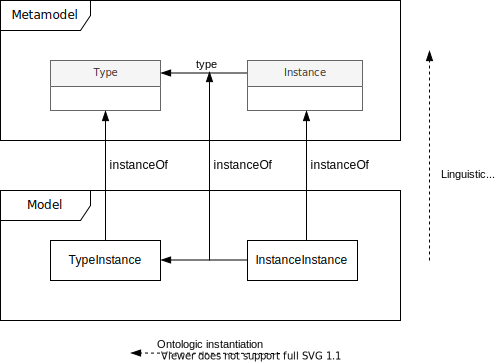
\includegraphics[width=1.0 \columnwidth]{Figures/Instantiation.pdf}
    \caption{Linguistic and ontologic instantiation}
    \label{fig:LinguisticAndOntologicInstantiation}
\end{figure}

\begin{figure}
    \centering
    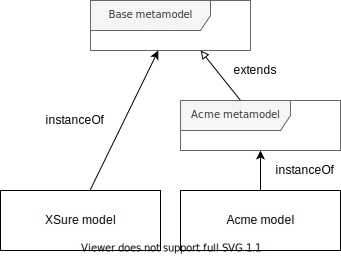
\includegraphics[width=0.7 \columnwidth]{Figures/MultilevelArchitecture.pdf}
    \caption{Multilevel architecture for the Process Challenge}
    \label{fig:MultilevelArchitecture}
\end{figure}




\section{Model presentation}
\label{sec:model}
detailed  presentation of a model, including justifications for design decisions


Sylvain

\section{Satisfaction of Requirements}
\label{sec:requirements}
%Satisfaction of Requirements: demonstration of how the solution satisfies the challenge requirements

In the previous section~\ref{sec:model}, we demonstrated that our solution satisfies all the challenge requirements. In this section, we summarize the different techniques used to satisfy them, without repeating all the justifications. We classify those techniques into three categories: 
\begin{itemize}
    \item \textbf{syntactic conformance}: the requirements are structurally satisfied when the model conforms to its metamodel,
    \item\textbf{constraints checking}: the requirements are fulfilled when all instances satisfy both syntactic conformance and the evaluation of invariants expressed for related concepts,
    \item \textbf{tooling}: the requirements are enforced by the implementation of the associated tooling.
\end{itemize}

Table \ref{tab:RequirementsSatisfactionBaseMetamodel} summarizes requirement covering for the base metamodel illustrated by XSure insurance use case while table \ref{tab:RequirementsSatisfactionAcme} shows requirements satisfaction for Acme software engineering process. Syntactic conformance is more precisely classified into six subcategories:

\begin{itemize}
    \item \textbf{Conceptualization} (\textit{Conc.}): a concept carries the semantics exposed by the requirement (for example for \textbf{P1}: \textit{process type} is conceptualized in a \textit{FlexoConcept} \textit{ProcessType}).
    \item \textbf{Specialization} (\textit{Spec.}): a concept is specialized in the sense of object-oriented modeling (for example for \textbf{P2}: \textit{Gateway} defines an abstract behavior \texttt{execute()} and \textit{Sequencing}, \textit{AndSplit}, \textit{AndJoin}, \textit{OrSplit} and \textit{OrJoin} are defined as inherited concepts implementing specific business logic).
    \item \textbf{Composition} (\textit{Comp.}): some concepts are in relation, or specific attributes were added to some concepts (for example for \textbf{P3}: a \textit{process type} has one \textit{initial task type}).
    \item \textbf{Linguistic instanciation} (\textit{L.Inst.}): requirement is satisfied by the instantiation of one or more concepts (for example for \textbf{S1}: \textit{requirement analysis} is defined as an instance of \textit{SETasktype}).
    \item \textbf{Ontologic instanciation} (\textit{O.Inst.}): fulfillment of requirement is obtained by the relation between an instance and its type definition instance (for example for \textbf{S3} : \textit{developer} has the dual concept nature in \textit{Acme metamodel} and instance nature in \textit{Acme model}).
    \item \textbf{Behavioral modeling} (\textit{B.Mod.}): requirement is satisfied by the definition of one more object-oriented behavioral features, which may combined with constraints checking and associated tooling (for example \textbf{P17}).
\end{itemize}

%Table~\ref{tab:RequirementsSatisfactionBaseMetamodel} 
%Table~\ref{tab:RequirementsSatisfactionAcme}

%Now we discuss how the solution satisfies the challenge requirements.

%\noteSylvain{
%Je voulais dire ici qu'on avait construit la solution pas à pas en suivant les requirements les uns après les autres, et qu'on avait à chaque fois veillé à traduire et respecter les requirements. Ca me semble très lourd de tout rejustifier ici.

%On peut cependant expliciter les différentes techniques employées:
%\begin{itemize}
%    \item Requirements satisfaits par conformance syntaxique: obligation de respecter le modèle structurel
%    \item Requirements satisfaits par ajout de contraintes: on peut instantier quelque chose de syntaxiquement correct, mais qui viole certaines contraintes (sur l'outillage les croix rouges)
%    \item Requirements satisfaits par l'outillage: ajout de comportements de manipulation du modèle qui "forcent" à respecter les contraintes d'intégrité resultant des requirements.
%\end{itemize}

%Peut-être peut-on faire un tableau qui rescence comment on a satisfait chaque contrainte ? Est ce que c'est %intéressant ?
%}
%\todo[inline]{OK pour le tableau synthétique +un petit peu de texte + une mini intro qui référence la section précédente (vu que les req ont été couverts dans la section précédente ; pas de fusion des deux sections}

%CT : Conceptualization
%SP : Specialization
%CP : Composition
%LI : Linguistic instantiation
%OI : Ontologic instantiation
%BM : behavioral modeling


\begin{figure*}
 \centering
\begin{tabular}{|c|c|c|c|c|c|c|c|c|}
   \hline
    & \multicolumn{6}{c|}{Syntactic conformance} & Constraints checking & Tooling\\
   \hline
                 & Conc.      & Spec.      & Comp.      & L.Inst.     & O.Inst.     & B.Mod.      &            & \\
  \hline
    \textbf{P1}  & \checkmark &            & \checkmark &            &            &            &            & \\
    \textbf{P2}  & \checkmark & \checkmark & \checkmark &            &            &            &            & \\
    \textbf{P3}  &            &            & \checkmark &            &            &            &            & \\
    \textbf{P4}  & \checkmark &            &            &            & \checkmark &            &            & \\
    \textbf{P5}  & \checkmark &            & \checkmark &            &            &            &            & \\
    \textbf{P6}  & \checkmark &            & \checkmark &            & \checkmark &            &            & \\
    \textbf{P7}  & \checkmark &            & \checkmark &            &            &            &            & \\
    \textbf{P8}  &            &            & \checkmark &            &            &            &            & \\
    \textbf{P9}  &            &            & \checkmark &            &            &            & \checkmark & \\
    \textbf{P10} & \checkmark &            &            &            & \checkmark &            &            & \\
    \textbf{P11} & \checkmark &            & \checkmark &            & \checkmark &            &            & \\
    \textbf{P12} &            &            & \checkmark &            &            &            &            & \\
    \textbf{P13} & \checkmark &            & \checkmark &            & \checkmark &            &            & \\
    \textbf{P14} & \checkmark &            &            &            & \checkmark &            &            & \\
    \textbf{P15} & \checkmark &            &            &            & \checkmark &            &            & \\
    \textbf{P16} & \checkmark &            &            &            & \checkmark &            &            & \\
    \textbf{P17} &            &            &            &            &            & \checkmark & \checkmark & \checkmark \\
    \textbf{P18} &            &            &            &            &            & \checkmark &            & \\
    \textbf{P19} &            & \checkmark & \checkmark &            &            & \checkmark &            & \\
  \hline
\end{tabular}
     \caption{Requirements satisfaction for base metamodel}
    \label{tab:RequirementsSatisfactionBaseMetamodel}
\end{figure*}

\begin{figure*}
 \centering
\begin{tabular}{|c|c|c|c|c|c|c|c|c|}
   \hline
    & \multicolumn{6}{c|}{Syntactic conformance} & Constraints checking & Tooling\\
   \hline
                 & Conc.      & Spec.      & Comp.      & L.Inst     & O.Inst     & B.Mod      &            & \\
  \hline
    \textbf{S1}  &            &            &            & \checkmark &            &            &            & \\
    \textbf{S2}  &            &            &            & \checkmark &            &            &            & \\
    \textbf{S3}  & \checkmark & \checkmark & \checkmark & \checkmark &            &            &            & \checkmark \\
    \textbf{S4}  & \checkmark & \checkmark & \checkmark & \checkmark &            &            &            & \\
    \textbf{S5}  &            & \checkmark &            & \checkmark &            & \checkmark &            & \\
    \textbf{S6}  &            & \checkmark &            & \checkmark &            & \checkmark & \checkmark & \\
    \textbf{S7}  &            &            &            & \checkmark &            & \checkmark &            & \\
    \textbf{S8}  &            &            &            & \checkmark &            &            &            & \\
    \textbf{S9}  &            &            &            &            &            & \checkmark & \checkmark & \\
    \textbf{S10} & \checkmark & \checkmark & \checkmark &            &            &            &            & \\
    \textbf{S11} &            &            &            & \checkmark &            &            &            & \checkmark \\
    \textbf{S12} &            &            &            & \checkmark &            &            &            & \checkmark \\
    \textbf{S13} &            &            &            & \checkmark &            &            &            & \\
  \hline
\end{tabular}
     \caption{Requirements satisfaction for Acme software engineering process}
    \label{tab:RequirementsSatisfactionAcme}
\end{figure*}


\section{Assessment of the Modeling Solution}
\label{sec:discussion}
discussing choices  made (ex : héritage vs attr), pointing out potential compromises/deficiencies
jc, fabien ; 
pas d'explicitation de niveaux de « concrétude » : conséquences ? facile de tracer des liens entre les niveaux ; difficile d'avoir le niveau ; 
outil adaptable, niveau d'abstraction, on fournit une solution + l'outil pour exécuter le processus ; réutilisabilité des modèles ; 
\todo[inline]{on pourrait aussi répondre ici aux 3 questions posées explicitement (copiées dansl'intro pour le moment), a priori non, le chef trouve que c'est chiant}

ajouter quelques métriquse "gros grains"

difficultés/facilités : contraintes faites à la main par rapport aux langages où on peut spécifier le niveau d'extension lorsque l'on trace un lien multi niveaux -> outil plus souple, mais moins de comportements automatisés ; + ouvert ; moins de support (faudrait implémenter ce qui manque) ; requiert de la méthode, ajouter des comportemets, etc.
points saillants :  outillage "gratuit" ; 



Although our tool was not designed with a focus on multi-level modelling, we were able to propose a fully working solution. 

Our approach is level-blind, therefore it is not easy to quickly retrieve the abstraction level of a concept.


\section{Related work}
\label{sec:relatedwork}
Positioning  and  contrasting  the  presented solution with related work

Salvador commence


\section{Conclusions}
\label{sec:conclusions}
%Conclusions: including  lessons  learned,  impulses  for future work, etc.

%\todo[inline]{lessons learned, impulse for future work -> fait émerger la question d'ajouter des bibliothèques dédiées au multi-niveaux (avoir des behaviors)}

We fulfill all the challenge requirements and we propose a tooling that demonstrates the usability of our solution.  We developed an ad-hoc solution, including models and metamodels, thanks to the flexibility provided by the metametamodeling infrastructure offered by Openflexo.

As a future work we envision to explore a number of alternative solutions: first, we intend to propose another approach based on a more agnostic level solution such as Clabjects. Instead of two levels defined by Type and Instance concepts, we could have a single concept mixing a type part and an instance part. This approach would probably be easier if specifications evolve. Secondly, another possible approach is the use of the free modeling tool proposed by Openflexo. The solution would be developed from examples (Acme and XSure processes for instance) from which models would be identified. Finally, the realisation of this challenge highlighted the interest of integrating specific behaviors for multi-level concepts management in Openflexo infrastructure, to avoid tailoring them, as in this exercise. We intend to do so.

\printbibliography

\end{article}

\end{document}
%%
